\documentclass[tikz,border=10pt]{standalone}
\usepackage{tikz}
\usepackage{amssymb}
\usetikzlibrary{shapes.geometric, arrows.meta, positioning, fit, backgrounds, calc}

\tikzset{
  startstop/.style={rectangle, rounded corners=22pt,
    minimum width=3.2cm, minimum height=1cm,
    text centered, draw=black!40, fill=gray!15,
    font=\small\bfseries},
  process/.style={rectangle, rounded corners=6pt,
    minimum width=5.5cm, minimum height=1.4cm,
    text centered, draw=black!40, fill=teal!12,
    font=\small\bfseries, align=center},
  decision/.style={rectangle, rounded corners=6pt,
    minimum width=5.5cm, minimum height=1.4cm,
    text centered, draw=black!40, fill=orange!18,
    font=\small\bfseries, align=center},
  action/.style={rectangle, rounded corners=6pt,
    minimum width=5.5cm, minimum height=1.4cm,
    text centered, draw=black!40, fill=red!12,
    font=\small\bfseries, align=center},
  sidenote/.style={rectangle, rounded corners=4pt,
    minimum width=1.6cm, minimum height=1.1cm,
    text centered, draw=black!30, fill=blue!12,
    font=\scriptsize\bfseries, align=center},
  sideaction/.style={rectangle, rounded corners=4pt,
    minimum width=2.2cm, minimum height=1.1cm,
    text centered, draw=black!30, fill=red!10,
    font=\scriptsize\bfseries, align=center},
  pagebox/.style={rectangle, rounded corners=4pt,
    minimum width=1.6cm, minimum height=1cm,
    text centered, draw=black!30, fill=blue!10,
    font=\scriptsize\bfseries, align=center},
  % Page action flowchart styles
  pagenode/.style={rectangle, rounded corners=6pt,
    minimum width=4.5cm, minimum height=1.3cm,
    text centered, draw=black!40, fill=teal!12,
    font=\small\bfseries, align=center},
  pagedecision/.style={rectangle, rounded corners=6pt,
    minimum width=4.5cm, minimum height=1.3cm,
    text centered, draw=black!40, fill=orange!18,
    font=\small\bfseries, align=center},
  pageaction/.style={rectangle, rounded corners=6pt,
    minimum width=4.5cm, minimum height=1.3cm,
    text centered, draw=black!40, fill=red!12,
    font=\small\bfseries, align=center},
  pageleaf/.style={rectangle, rounded corners=6pt,
    minimum width=3.2cm, minimum height=1.1cm,
    text centered, draw=black!30, fill=blue!10,
    font=\scriptsize\bfseries, align=center},
  arr/.style={-{Stealth[length=6pt]}, thick, draw=black!50},
  loopline/.style={draw=black!35, thick},
}

\begin{document}

%===========================================
% FLOWCHART 1: Main loop
%===========================================
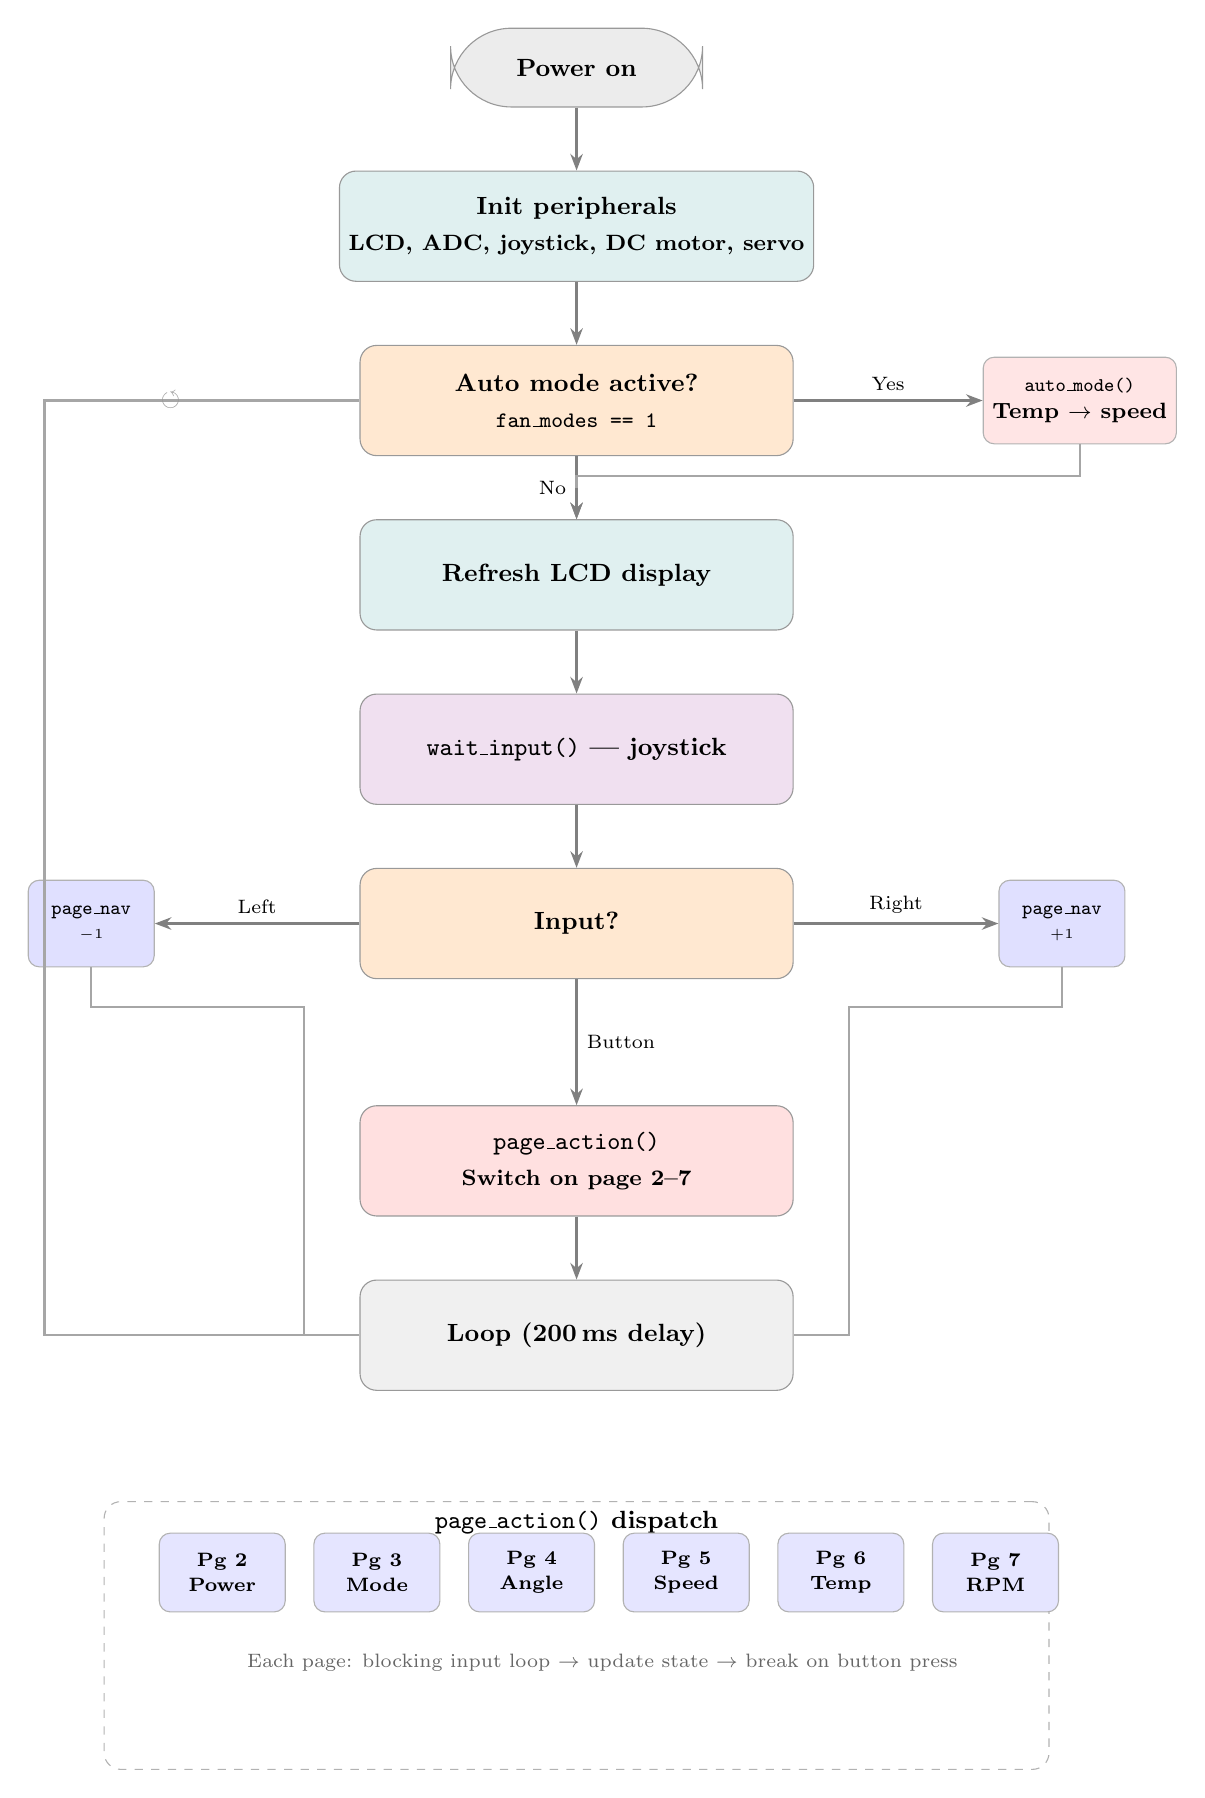
\begin{tikzpicture}[node distance=0.8cm and 2.0cm]

\node (start) [startstop]
  {Power on};

\node (init) [process, below=of start]
  {Init peripherals\\[2pt]
   {\footnotesize LCD, ADC, joystick, DC motor, servo}};

\node (autoq) [decision, below=of init]
  {Auto mode active?\\[2pt]
   {\footnotesize \texttt{fan\_modes == 1}}};

\node (lcd) [process, below=of autoq]
  {Refresh LCD display};

\node (waitin) [process, below=of lcd, fill=violet!12]
  {\texttt{wait\_input()} --- joystick};

\node (inputq) [decision, below=of waitin]
  {Input?};

\node (paction) [action, below=1.6cm of inputq]
  {\texttt{page\_action()}\\[2pt]
   {\footnotesize Switch on page 2--7}};

\node (loopend) [process, below=of paction, fill=gray!12]
  {Loop (200\,ms delay)};

\node (autoact) [sideaction, right=2.4cm of autoq]
  {\texttt{auto\_mode()}\\[2pt]
   {\footnotesize Temp $\to$ speed}};

\node (navl) [sidenote, left=2.6cm of inputq]
  {\texttt{page\_nav}\\[1pt] {\tiny $-1$}};

\node (navr) [sidenote, right=2.6cm of inputq]
  {\texttt{page\_nav}\\[1pt] {\tiny $+1$}};

\draw[arr] (start)   -- (init);
\draw[arr] (init)    -- (autoq);
\draw[arr] (autoq)   -- node[left,  font=\scriptsize]{No} (lcd);
\draw[arr] (lcd)     -- (waitin);
\draw[arr] (waitin)  -- (inputq);
\draw[arr] (inputq)  -- node[right, font=\scriptsize]{Button} (paction);
\draw[arr] (paction) -- (loopend);

\draw[arr] (autoq.east) -- node[above, font=\scriptsize]{Yes} (autoact.west);
\draw[loopline] (autoact.south) -- ++(0,-0.4) -| ($(lcd.north)+(0,0.4)$);
\draw[arr] ($(lcd.north)+(0,0.4)$) -- (lcd.north);

\draw[arr] (inputq.west) -- node[above, font=\scriptsize]{Left}  (navl.east);
\draw[loopline] (navl.south) -- ++(0,-0.5) -| ($(loopend.west)+(-0.7,0)$) -- (loopend.west);

\draw[arr] (inputq.east) -- node[above, font=\scriptsize]{Right} (navr.west);
\draw[loopline] (navr.south) -- ++(0,-0.5) -| ($(loopend.east)+(0.7,0)$) -- (loopend.east);

\draw[loopline] (loopend.west) -- ++(-4.0,0) |- (autoq.west);
\node[font=\small, text=black!40] at ($(autoq.west)+(-2.4,0)$) {$\circlearrowleft$};

\node (leg) [draw=black!30, dashed, rounded corners=6pt,
             below=1.4cm of loopend,
             minimum width=12cm, minimum height=3.4cm,
             label={[font=\small\bfseries, anchor=north]north:\texttt{page\_action()} dispatch}] {};

\node (p2) [pagebox, below=1.8cm of loopend, xshift=-4.5cm] {Pg 2\\[1pt] Power};
\node (p3) [pagebox, right=0.35cm of p2]  {Pg 3\\[1pt] Mode};
\node (p4) [pagebox, right=0.35cm of p3]  {Pg 4\\[1pt] Angle};
\node (p5) [pagebox, right=0.35cm of p4]  {Pg 5\\[1pt] Speed};
\node (p6) [pagebox, right=0.35cm of p5]  {Pg 6\\[1pt] Temp};
\node (p7) [pagebox, right=0.35cm of p6]  {Pg 7\\[1pt] RPM};

\node[font=\scriptsize, text=black!60, below=0.4cm of p4, xshift=0.9cm]
  {Each page: blocking input loop $\to$ update state $\to$ break on button press};

\end{tikzpicture}

\bigskip

%===========================================
% FLOWCHART 2: page_action() detail
%===========================================
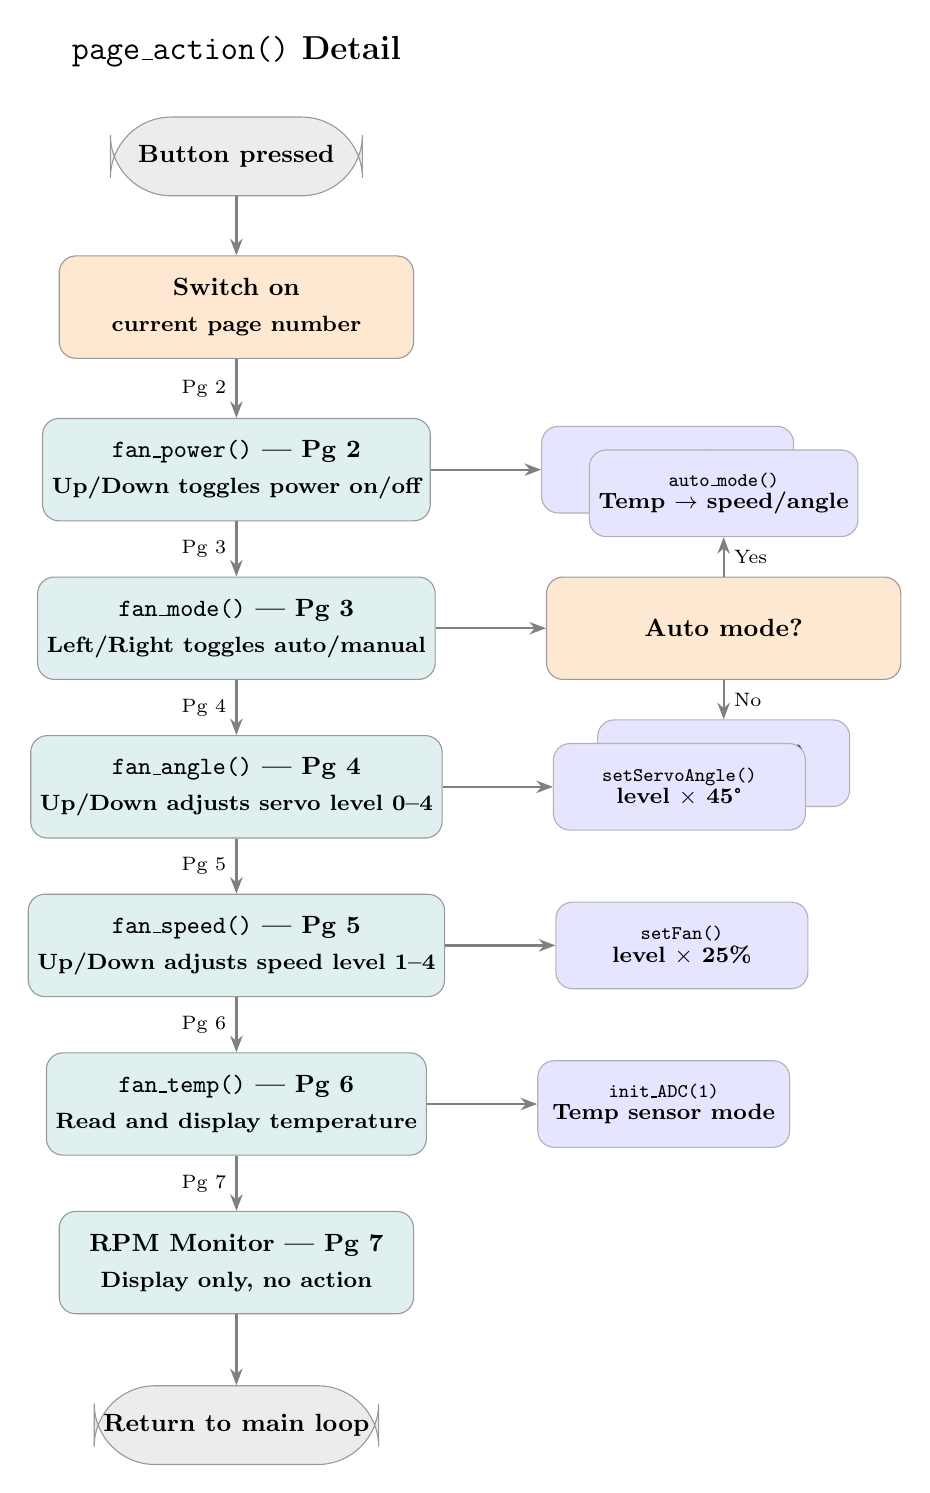
\begin{tikzpicture}[node distance=0.75cm and 1.6cm]

% Title
\node (title) [font=\large\bfseries] {\texttt{page\_action()} Detail};

% Entry
\node (entry) [startstop, below=0.5cm of title]
  {Button pressed};

\node (sw) [pagedecision, below=of entry]
  {Switch on\\[2pt] {\footnotesize current page number}};

% Page 2
\node (pg2) [pagenode, below=of sw]
  {\texttt{fan\_power()} --- Pg 2\\[2pt]
   {\footnotesize Up/Down toggles power on/off}};

\node (pg2a) [pageleaf, right=1.4cm of pg2]
  {\texttt{startFan()}\\or \texttt{stopFan()}};

\draw[arr] (pg2.east) -- (pg2a.west);

% Page 3
\node (pg3) [pagenode, below=0.7cm of pg2]
  {\texttt{fan\_mode()} --- Pg 3\\[2pt]
   {\footnotesize Left/Right toggles auto/manual}};

\node (pg3q) [pagedecision, right=1.4cm of pg3]
  {Auto mode?};

\node (pg3y) [pageleaf, above=0.5cm of pg3q]
  {\texttt{auto\_mode()}\\{\footnotesize Temp $\to$ speed/angle}};

\node (pg3n) [pageleaf, below=0.5cm of pg3q]
  {\texttt{servoOscilate(0)}\\{\footnotesize Reset to 90\textdegree}};

\draw[arr] (pg3.east)   -- (pg3q.west);
\draw[arr] (pg3q.north) -- node[right, font=\scriptsize]{Yes} (pg3y.south);
\draw[arr] (pg3q.south) -- node[right, font=\scriptsize]{No}  (pg3n.north);

% Page 4
\node (pg4) [pagenode, below=0.7cm of pg3]
  {\texttt{fan\_angle()} --- Pg 4\\[2pt]
   {\footnotesize Up/Down adjusts servo level 0--4}};

\node (pg4a) [pageleaf, right=1.4cm of pg4]
  {\texttt{setServoAngle()}\\{\footnotesize level $\times$ 45\textdegree}};

\draw[arr] (pg4.east) -- (pg4a.west);

% Page 5
\node (pg5) [pagenode, below=0.7cm of pg4]
  {\texttt{fan\_speed()} --- Pg 5\\[2pt]
   {\footnotesize Up/Down adjusts speed level 1--4}};

\node (pg5a) [pageleaf, right=1.4cm of pg5]
  {\texttt{setFan()}\\{\footnotesize level $\times$ 25\%}};

\draw[arr] (pg5.east) -- (pg5a.west);

% Page 6
\node (pg6) [pagenode, below=0.7cm of pg5]
  {\texttt{fan\_temp()} --- Pg 6\\[2pt]
   {\footnotesize Read and display temperature}};

\node (pg6a) [pageleaf, right=1.4cm of pg6]
  {\texttt{init\_ADC(1)}\\{\footnotesize Temp sensor mode}};

\draw[arr] (pg6.east) -- (pg6a.west);

% Page 7
\node (pg7) [pagenode, below=0.7cm of pg6]
  {RPM Monitor --- Pg 7\\[2pt]
   {\footnotesize Display only, no action}};

% Return
\node (ret) [startstop, below=0.9cm of pg7]
  {Return to main loop};

% Spine arrows
\draw[arr] (entry) -- (sw);
\draw[arr] (sw)    -- node[left, font=\scriptsize]{Pg 2} (pg2);
\draw[arr] (pg2)   -- node[left, font=\scriptsize]{Pg 3} (pg3);
\draw[arr] (pg3)   -- node[left, font=\scriptsize]{Pg 4} (pg4);
\draw[arr] (pg4)   -- node[left, font=\scriptsize]{Pg 5} (pg5);
\draw[arr] (pg5)   -- node[left, font=\scriptsize]{Pg 6} (pg6);
\draw[arr] (pg6)   -- node[left, font=\scriptsize]{Pg 7} (pg7);
\draw[arr] (pg7)   -- (ret);

\end{tikzpicture}

\end{document}